\documentclass[]{elsarticle} %review=doublespace preprint=single 5p=2 column
%%% Begin My package additions %%%%%%%%%%%%%%%%%%%
\usepackage[hyphens]{url}
\usepackage{lineno} % add
\providecommand{\tightlist}{%
  \setlength{\itemsep}{0pt}\setlength{\parskip}{0pt}}

\bibliographystyle{elsarticle-harv}
\biboptions{sort&compress} % For natbib
\usepackage{graphicx}
\usepackage{booktabs} % book-quality tables
%% Redefines the elsarticle footer
%\makeatletter
%\def\ps@pprintTitle{%
% \let\@oddhead\@empty
% \let\@evenhead\@empty
% \def\@oddfoot{\it \hfill\today}%
% \let\@evenfoot\@oddfoot}
%\makeatother

% A modified page layout
\textwidth 6.75in
\oddsidemargin -0.15in
\evensidemargin -0.15in
\textheight 9in
\topmargin -0.5in
%%%%%%%%%%%%%%%% end my additions to header

\usepackage[T1]{fontenc}
\usepackage{lmodern}
\usepackage{amssymb,amsmath}
\usepackage{ifxetex,ifluatex}
\usepackage{fixltx2e} % provides \textsubscript
% use upquote if available, for straight quotes in verbatim environments
\IfFileExists{upquote.sty}{\usepackage{upquote}}{}
\ifnum 0\ifxetex 1\fi\ifluatex 1\fi=0 % if pdftex
  \usepackage[utf8]{inputenc}
\else % if luatex or xelatex
  \usepackage{fontspec}
  \ifxetex
    \usepackage{xltxtra,xunicode}
  \fi
  \defaultfontfeatures{Mapping=tex-text,Scale=MatchLowercase}
  \newcommand{\euro}{€}
\fi
% use microtype if available
\IfFileExists{microtype.sty}{\usepackage{microtype}}{}
\usepackage{longtable}
\usepackage{graphicx}
% We will generate all images so they have a width \maxwidth. This means
% that they will get their normal width if they fit onto the page, but
% are scaled down if they would overflow the margins.
\makeatletter
\def\maxwidth{\ifdim\Gin@nat@width>\linewidth\linewidth
\else\Gin@nat@width\fi}
\makeatother
\let\Oldincludegraphics\includegraphics
\renewcommand{\includegraphics}[1]{\Oldincludegraphics[width=\maxwidth]{#1}}
\ifxetex
  \usepackage[setpagesize=false, % page size defined by xetex
              unicode=false, % unicode breaks when used with xetex
              xetex]{hyperref}
\else
  \usepackage[unicode=true]{hyperref}
\fi
\hypersetup{breaklinks=true,
            bookmarks=true,
            pdfauthor={},
            pdftitle={A simplified dynamic bioenergetic model for coral-algal symbiosis and coral bleaching},
            colorlinks=true,
            urlcolor=blue,
            linkcolor=magenta,
            pdfborder={0 0 0}}
\urlstyle{same}  % don't use monospace font for urls
\setlength{\parindent}{0pt}
\setlength{\parskip}{6pt plus 2pt minus 1pt}
\setlength{\emergencystretch}{3em}  % prevent overfull lines
\setcounter{secnumdepth}{0}
% Pandoc toggle for numbering sections (defaults to be off)
\setcounter{secnumdepth}{0}
% Pandoc header


\usepackage[nomarkers]{endfloat}

\begin{document}
\begin{frontmatter}

  \title{A simplified dynamic bioenergetic model for coral-algal symbiosis and
coral bleaching}
    \author[University of Hawaii]{Ross Cunning\corref{c1}}
   \ead{ross.cunning@gmail.com} 
   \cortext[c1]{Corresponding Author}
    \author[University of California]{Erik B. Muller}
  
  
    \author[University of Hawaii]{Ruth D. Gates}
  
  
    \author[University of California]{Roger M. Nisbet}
  
  
      \address[University of Hawaii]{Hawaii Institute of Marine Biology, Kaneohe, HI 96744, USA}
    \address[University of California]{Department of Ecology, Evolution, and Marine Biology, Santa Barbara, CA
93106, USA}
  
  \begin{abstract}
  This is the abstract. Some type of positive feedback is necessary.
  Compare scenarios of recycling CO2, have photodamage increase
  maintenance that does recycle CO2. Compare recycled N to symbiont
  instead of host How much do you have to reduce the light to get
  recovery? i.e., magnitude of hysteresis?
  \end{abstract}
  
 \end{frontmatter}

\section{Introduction}\label{introduction}

The nutritional exchange between corals and \emph{Symbiodinium} directly
underlies the capacity of corals to build coral reef ecosystems, worth
trillions of US Dollars annually (Costanza, Groot, and Sutton 2014).
However, the complex symbiotic metabolism of corals is vulnerable to
disruption by numerous anthropogenic environmental perturbations,
jeopardizing their future persistence. In order to understand and
predict coral responses to complex changes in their environment, a
mechanistic understanding of how multiple interacting factors drive the
individual and emergent physiology of both symbiotic partners is
necessary. Such a task is well suited for theoretical modeling
frameworks such as Dynamic Energy Budget (DEB) theory (Kooijman 2010),
although the complexity of such theory makes these efforts inaccessible
to many biologists (Jager, Martin, and Zimmer 2013). In order to bridge
this gap, we present here a simplified dynamic bioenergetic model for
coral-\emph{Symbiodinium} symbioses that aims to mechanistically
integrate the impacts of complex environmental change on the
physiological performance of reef corals, including responses to
environmental stress.

In reef coral symbioses, intracellular \emph{Symbiodinium} translocate
photosynthetically fixed carbon to support coral metabolism, while the
animal host provides access to inorganic nutrients and carbon dioxide
(Muscatine and Porter 1977). Previous application of DEB theory to this
syntrophic system (Muller et al. 2009) demonstrated a stable symbiotic
relationship and qualitatively realistic growth and biomass ratios
across gradients of ambient irradiance, nutrients, and food. This model
assumed that 1) \emph{Symbiodinium} has priority access to fixed carbon
through photosynthesis, 2) the coral animal has priority access to
dissolved nitrogen through contact with seawater, and 3) each partner
shares with the other only what it cannot use for its own growth. In its
simplest form, this principle of sharing the surplus is sufficient to
describe the dynamics of diverse syntrophic organs and organisms (e.g.,
trees, duckweeds, corals), suggesting the mechanism is mathematically
and evolutionarily robust (Nisbet et al., in prep.).

While the formal DEB model of Muller et al. (2009) represents the most
significant theoretical contribution in coral symbiosis research to
date, we aim to strengthen the role of theory and broaden its potential
application in three primary ways:

\begin{enumerate}
\def\labelenumi{\arabic{enumi}.}
\item
  \emph{Develop a detailed module of environmental stress.} Of primary
  interest to coral biologists and ecologists is symbiosis dysfunction
  under environmental stress, resulting in coral ``bleaching''--the loss
  of algal symbionts from the association (Jokiel and Coles 1977).
  Photooxidative stress in \emph{Symbiodinium} is considered a primary
  trigger of bleaching in response to high temperature and/or light
  (Weis 2008), and prolonged or severe bleaching can result in
  mortality, though corals sometimes recover their symbionts. Bleaching
  susceptibility, severity, and recovery may by influenced by
  interacting factors such as heterotrophy and nutrient availability
  (Wooldridge 2014b), and the genetic identity of \emph{Symbiodinium}
  (Glynn et al. 2001). To simulate these bleaching-related phenomena, we
  develop a generalized framework linking overreduction of the
  photosynthetic light reactions to downstream impacts of
  photoinhibition and photodamage.
\item
  \emph{Reduce theoretical and mathematical complexity.} Following the
  logic of Jager, Martin, and Zimmer (2013), we exclude certain features
  of formal DEB models in order to capture behaviors of interest with
  the simplest possible formulation. Here, we present a model without
  reserves, maturity, or reproduction (see Kooijman 2010). This
  formulation restricts the model's scope to the bioenergetics of growth
  and symbiosis dynamics in adult corals (i.e., reproduction, larval
  stages, and metamorphosis are not considered), but greatly reduces
  theoretical complexity and parameter numbers, which is advantageous
  given the relative paucity of data for corals. However, our primary
  motivation for reducing complexity was to increase accessibility and
  applicability for biologists and ecologists without requiring
  significant expertise in DEB theory.
\item
  \emph{Provide well-documented, open-access code.} In order to
  facilitate the continued development and application of theoretical
  modeling tools for coral symbioses, we provide open access to the
  model in the form of detailed, commented code written in the R
  language (R Core Team 2014). With an accessible and modular framework,
  we envision this as a resource for futher development by the
  scientific community to include additional complexity and
  problem-specific components. To widen the audience for this work, we
  chose the R language because it is freely available and in common use
  by biologists and ecologists.
\end{enumerate}

With these as our primary motivations, we describe a simplified approach
to dynamic bioenergetic modeling of coral-algal symbioses that tracks
carbon and nitrogen acquisition and sharing between partners. This
theoretical framework dynamically integrates the influence of external
irradiance, nutrients, and prey availability on coral growth and
symbiosis dynamics (i.e., symbiont:host biomass ratios), allowing for
the possibility of coral bleaching in the event of photooxidative
stress. In the following sections, we describe the formulation of this
model and justify its structure and parameter values based on relevant
literature. We then demonstrate the model's behavior and discuss some of
its major implications and outcomes, and the wide range of potential
applications for this model in the study of cnidarian-algal symbioses.

\section{Model description}\label{model-description}

In this dynamic bioenergetic model of coral-algal symbiosis, carbon and
nitrogen are acquired by each partner and used to construct biomass. A
graphical representation of the model is presented in Fig. 1, and each
model flux and parameter are defined in Tables 1 and 2, respectively. We
use C-moles as the unit of biomass for consistency with the rigorous
mass balance of DEB theory: 1 C-mole is equivalent to the amount of
biomass containing 1 mole of Carbon atoms. Host biomass (\(H\)),
symbiont biomass (\(S\)), and prey biomass (\(X\)) have fixed, but
different, molar N:C ratios (Table 2). Carbon and nitrogen are combined
to produce biomass by synthesizing units (SU), which are mathematical
specifications of the formation of a product from two substrates; we use
the parallel complementary formulation of Kooijman (2010) to specify
these fluxes. The two state variables are symbiont biomass and coral
biomass; because resources are acquired proportionally to surface area,
and surface area is proportional to volume (i.e., corals are
``V1-morphs'' in DEB terminology (Kooijman 2010)), biomass increases
exponentially during growth (indeed, corals grow exponentially (Bak
1976)). The specific growth rate and the ratio of symbiont to host
biomass are the responses of interest of the system. Below we describe
the formulation of each flux involved in producing these responses.

Table 1. Model fluxes

\begin{longtable}[c]{@{}llll@{}}
\toprule
\begin{minipage}[b]{0.12\columnwidth}\raggedright\strut
Symbol
\strut\end{minipage} &
\begin{minipage}[b]{0.48\columnwidth}\raggedright\strut
Description
\strut\end{minipage} &
\begin{minipage}[b]{0.26\columnwidth}\raggedright\strut
Units
\strut\end{minipage} &
\begin{minipage}[b]{0.10\columnwidth}\raggedright\strut
Eq. no.
\strut\end{minipage}\tabularnewline
\midrule
\endhead
\begin{minipage}[t]{0.12\columnwidth}\raggedright\strut
\(j_X\)
\strut\end{minipage} &
\begin{minipage}[t]{0.48\columnwidth}\raggedright\strut
Prey uptake rate
\strut\end{minipage} &
\begin{minipage}[t]{0.26\columnwidth}\raggedright\strut
molX CmolH\textsuperscript{-1} d\textsuperscript{-1}
\strut\end{minipage} &
\begin{minipage}[t]{0.10\columnwidth}\raggedright\strut
3
\strut\end{minipage}\tabularnewline
\begin{minipage}[t]{0.12\columnwidth}\raggedright\strut
\(j_N\)
\strut\end{minipage} &
\begin{minipage}[t]{0.48\columnwidth}\raggedright\strut
Nitrogen uptake rate
\strut\end{minipage} &
\begin{minipage}[t]{0.26\columnwidth}\raggedright\strut
molN CmolH\textsuperscript{-1} d\textsuperscript{-1}
\strut\end{minipage} &
\begin{minipage}[t]{0.10\columnwidth}\raggedright\strut
4
\strut\end{minipage}\tabularnewline
\begin{minipage}[t]{0.12\columnwidth}\raggedright\strut
\(j_{HG}\)
\strut\end{minipage} &
\begin{minipage}[t]{0.48\columnwidth}\raggedright\strut
Host biomass formation rate
\strut\end{minipage} &
\begin{minipage}[t]{0.26\columnwidth}\raggedright\strut
CmolH CmolH\textsuperscript{-1} d\textsuperscript{-1}
\strut\end{minipage} &
\begin{minipage}[t]{0.10\columnwidth}\raggedright\strut
5
\strut\end{minipage}\tabularnewline
\begin{minipage}[t]{0.12\columnwidth}\raggedright\strut
\(r_{NH}\)
\strut\end{minipage} &
\begin{minipage}[t]{0.48\columnwidth}\raggedright\strut
Recycled nitrogen from host turnover
\strut\end{minipage} &
\begin{minipage}[t]{0.26\columnwidth}\raggedright\strut
molN CmolH\textsuperscript{-1} d\textsuperscript{-1}
\strut\end{minipage} &
\begin{minipage}[t]{0.10\columnwidth}\raggedright\strut
6
\strut\end{minipage}\tabularnewline
\begin{minipage}[t]{0.12\columnwidth}\raggedright\strut
\(\rho_N\)
\strut\end{minipage} &
\begin{minipage}[t]{0.48\columnwidth}\raggedright\strut
Nitrogen shared with the symbiont
\strut\end{minipage} &
\begin{minipage}[t]{0.26\columnwidth}\raggedright\strut
molN CmolH\textsuperscript{-1} d\textsuperscript{-1}
\strut\end{minipage} &
\begin{minipage}[t]{0.10\columnwidth}\raggedright\strut
7
\strut\end{minipage}\tabularnewline
\begin{minipage}[t]{0.12\columnwidth}\raggedright\strut
\(j_{eC}\)
\strut\end{minipage} &
\begin{minipage}[t]{0.48\columnwidth}\raggedright\strut
Excess carbon used to activate host CCMs
\strut\end{minipage} &
\begin{minipage}[t]{0.26\columnwidth}\raggedright\strut
molC CmolH\textsuperscript{-1} d\textsuperscript{-1}
\strut\end{minipage} &
\begin{minipage}[t]{0.10\columnwidth}\raggedright\strut
\strut\end{minipage}\tabularnewline
\begin{minipage}[t]{0.12\columnwidth}\raggedright\strut
\(j_L\)
\strut\end{minipage} &
\begin{minipage}[t]{0.48\columnwidth}\raggedright\strut
Light absorption rate
\strut\end{minipage} &
\begin{minipage}[t]{0.26\columnwidth}\raggedright\strut
molph CmolS\textsuperscript{-1} d\textsuperscript{-1}
\strut\end{minipage} &
\begin{minipage}[t]{0.10\columnwidth}\raggedright\strut
9
\strut\end{minipage}\tabularnewline
\begin{minipage}[t]{0.12\columnwidth}\raggedright\strut
\(j_{CO_2}\)
\strut\end{minipage} &
\begin{minipage}[t]{0.48\columnwidth}\raggedright\strut
CO\textsubscript{2} input to photosynthesis
\strut\end{minipage} &
\begin{minipage}[t]{0.26\columnwidth}\raggedright\strut
molCO\textsubscript{2} CmolH\textsuperscript{-1} d\textsuperscript{-1}
\strut\end{minipage} &
\begin{minipage}[t]{0.10\columnwidth}\raggedright\strut
10
\strut\end{minipage}\tabularnewline
\begin{minipage}[t]{0.12\columnwidth}\raggedright\strut
\(r_{CH}\)
\strut\end{minipage} &
\begin{minipage}[t]{0.48\columnwidth}\raggedright\strut
Recycled CO\textsubscript{2} from host turnover
\strut\end{minipage} &
\begin{minipage}[t]{0.26\columnwidth}\raggedright\strut
molCO\textsubscript{2} CmolH\textsuperscript{-1} d\textsuperscript{-1}
\strut\end{minipage} &
\begin{minipage}[t]{0.10\columnwidth}\raggedright\strut
11
\strut\end{minipage}\tabularnewline
\begin{minipage}[t]{0.12\columnwidth}\raggedright\strut
\(r_{CS}\)
\strut\end{minipage} &
\begin{minipage}[t]{0.48\columnwidth}\raggedright\strut
Recycled CO\textsubscript{2} from symbiont turnover
\strut\end{minipage} &
\begin{minipage}[t]{0.26\columnwidth}\raggedright\strut
molCO\textsubscript{2} CmolS\textsuperscript{-1} d\textsuperscript{-1}
\strut\end{minipage} &
\begin{minipage}[t]{0.10\columnwidth}\raggedright\strut
12
\strut\end{minipage}\tabularnewline
\begin{minipage}[t]{0.12\columnwidth}\raggedright\strut
\(j_{CP}\)
\strut\end{minipage} &
\begin{minipage}[t]{0.48\columnwidth}\raggedright\strut
Photosynthesis rate
\strut\end{minipage} &
\begin{minipage}[t]{0.26\columnwidth}\raggedright\strut
molC CmolS\textsuperscript{-1} d\textsuperscript{-1}
\strut\end{minipage} &
\begin{minipage}[t]{0.10\columnwidth}\raggedright\strut
13
\strut\end{minipage}\tabularnewline
\begin{minipage}[t]{0.12\columnwidth}\raggedright\strut
\(j_{eL}\)
\strut\end{minipage} &
\begin{minipage}[t]{0.48\columnwidth}\raggedright\strut
Light energy in excess of photochemistry
\strut\end{minipage} &
\begin{minipage}[t]{0.26\columnwidth}\raggedright\strut
molph CmolS\textsuperscript{-1} d\textsuperscript{-1}
\strut\end{minipage} &
\begin{minipage}[t]{0.10\columnwidth}\raggedright\strut
14
\strut\end{minipage}\tabularnewline
\begin{minipage}[t]{0.12\columnwidth}\raggedright\strut
\(j_{NPQ}\)
\strut\end{minipage} &
\begin{minipage}[t]{0.48\columnwidth}\raggedright\strut
Total capacity of NPQ
\strut\end{minipage} &
\begin{minipage}[t]{0.26\columnwidth}\raggedright\strut
molph CmolS\textsuperscript{-1} d\textsuperscript{-1}
\strut\end{minipage} &
\begin{minipage}[t]{0.10\columnwidth}\raggedright\strut
15
\strut\end{minipage}\tabularnewline
\begin{minipage}[t]{0.12\columnwidth}\raggedright\strut
\(c_{ROS}\)
\strut\end{minipage} &
\begin{minipage}[t]{0.48\columnwidth}\raggedright\strut
ROS production proportional to baseline
\strut\end{minipage} &
\begin{minipage}[t]{0.26\columnwidth}\raggedright\strut
--
\strut\end{minipage} &
\begin{minipage}[t]{0.10\columnwidth}\raggedright\strut
16
\strut\end{minipage}\tabularnewline
\begin{minipage}[t]{0.12\columnwidth}\raggedright\strut
\(r_{NS}\)
\strut\end{minipage} &
\begin{minipage}[t]{0.48\columnwidth}\raggedright\strut
Recycled nitrogen from symbiont turnover
\strut\end{minipage} &
\begin{minipage}[t]{0.26\columnwidth}\raggedright\strut
molN CmolS\textsuperscript{-1} d\textsuperscript{-1}
\strut\end{minipage} &
\begin{minipage}[t]{0.10\columnwidth}\raggedright\strut
17
\strut\end{minipage}\tabularnewline
\begin{minipage}[t]{0.12\columnwidth}\raggedright\strut
\(j_{SG}\)
\strut\end{minipage} &
\begin{minipage}[t]{0.48\columnwidth}\raggedright\strut
Symbiont biomass formation rate
\strut\end{minipage} &
\begin{minipage}[t]{0.26\columnwidth}\raggedright\strut
CmolS CmolS\textsuperscript{-1} d\textsuperscript{-1}
\strut\end{minipage} &
\begin{minipage}[t]{0.10\columnwidth}\raggedright\strut
18
\strut\end{minipage}\tabularnewline
\begin{minipage}[t]{0.12\columnwidth}\raggedright\strut
\(\rho_C\)
\strut\end{minipage} &
\begin{minipage}[t]{0.48\columnwidth}\raggedright\strut
Fixed carbon shared with host
\strut\end{minipage} &
\begin{minipage}[t]{0.26\columnwidth}\raggedright\strut
molC CmolS\textsuperscript{-1} d\textsuperscript{-1}
\strut\end{minipage} &
\begin{minipage}[t]{0.10\columnwidth}\raggedright\strut
19
\strut\end{minipage}\tabularnewline
\begin{minipage}[t]{0.12\columnwidth}\raggedright\strut
\(j_{ST}\)
\strut\end{minipage} &
\begin{minipage}[t]{0.48\columnwidth}\raggedright\strut
Symbiont turnover rate
\strut\end{minipage} &
\begin{minipage}[t]{0.26\columnwidth}\raggedright\strut
CmolS CmolS\textsuperscript{-1} d\textsuperscript{-1}
\strut\end{minipage} &
\begin{minipage}[t]{0.10\columnwidth}\raggedright\strut
20
\strut\end{minipage}\tabularnewline
\bottomrule
\end{longtable}

Table 2. Model parameters

\begin{longtable}[c]{@{}llll@{}}
\toprule
\begin{minipage}[b]{0.10\columnwidth}\raggedright\strut
Symbol
\strut\end{minipage} &
\begin{minipage}[b]{0.48\columnwidth}\raggedright\strut
Description
\strut\end{minipage} &
\begin{minipage}[b]{0.09\columnwidth}\raggedright\strut
Value
\strut\end{minipage} &
\begin{minipage}[b]{0.23\columnwidth}\raggedright\strut
Units
\strut\end{minipage}\tabularnewline
\midrule
\endhead
\begin{minipage}[t]{0.10\columnwidth}\raggedright\strut
\(n_{NH}\)
\strut\end{minipage} &
\begin{minipage}[t]{0.48\columnwidth}\raggedright\strut
N:C molar ratio in host biomass
\strut\end{minipage} &
\begin{minipage}[t]{0.09\columnwidth}\raggedright\strut
0.19
\strut\end{minipage} &
\begin{minipage}[t]{0.23\columnwidth}\raggedright\strut
--
\strut\end{minipage}\tabularnewline
\begin{minipage}[t]{0.10\columnwidth}\raggedright\strut
\(n_{NS}\)
\strut\end{minipage} &
\begin{minipage}[t]{0.48\columnwidth}\raggedright\strut
N:C molar ratio in symbiont biomass
\strut\end{minipage} &
\begin{minipage}[t]{0.09\columnwidth}\raggedright\strut
0.2
\strut\end{minipage} &
\begin{minipage}[t]{0.23\columnwidth}\raggedright\strut
--
\strut\end{minipage}\tabularnewline
\begin{minipage}[t]{0.10\columnwidth}\raggedright\strut
\(n_{NX}\)
\strut\end{minipage} &
\begin{minipage}[t]{0.48\columnwidth}\raggedright\strut
N:C molar ratio in prey biomass
\strut\end{minipage} &
\begin{minipage}[t]{0.09\columnwidth}\raggedright\strut
0.13
\strut\end{minipage} &
\begin{minipage}[t]{0.23\columnwidth}\raggedright\strut
--
\strut\end{minipage}\tabularnewline
\begin{minipage}[t]{0.10\columnwidth}\raggedright\strut
\(j_{HT}^0\)
\strut\end{minipage} &
\begin{minipage}[t]{0.48\columnwidth}\raggedright\strut
Specific turnover rate of host biomass
\strut\end{minipage} &
\begin{minipage}[t]{0.09\columnwidth}\raggedright\strut
0.03
\strut\end{minipage} &
\begin{minipage}[t]{0.23\columnwidth}\raggedright\strut
CmolH CmolH\textsuperscript{-1} d\textsuperscript{-1}
\strut\end{minipage}\tabularnewline
\begin{minipage}[t]{0.10\columnwidth}\raggedright\strut
\(j_{ST}^0\)
\strut\end{minipage} &
\begin{minipage}[t]{0.48\columnwidth}\raggedright\strut
Specific turnover rate of symbiont biomass
\strut\end{minipage} &
\begin{minipage}[t]{0.09\columnwidth}\raggedright\strut
0.03
\strut\end{minipage} &
\begin{minipage}[t]{0.23\columnwidth}\raggedright\strut
CmolS CmolS\textsuperscript{-1} d\textsuperscript{-1}
\strut\end{minipage}\tabularnewline
\begin{minipage}[t]{0.10\columnwidth}\raggedright\strut
\(\sigma_{NH}\)
\strut\end{minipage} &
\begin{minipage}[t]{0.48\columnwidth}\raggedright\strut
Proportion host nitrogen turnover recycled
\strut\end{minipage} &
\begin{minipage}[t]{0.09\columnwidth}\raggedright\strut
0.9
\strut\end{minipage} &
\begin{minipage}[t]{0.23\columnwidth}\raggedright\strut
--
\strut\end{minipage}\tabularnewline
\begin{minipage}[t]{0.10\columnwidth}\raggedright\strut
\(\sigma_{CH}\)
\strut\end{minipage} &
\begin{minipage}[t]{0.48\columnwidth}\raggedright\strut
Proportion host carbon turnover recycled
\strut\end{minipage} &
\begin{minipage}[t]{0.09\columnwidth}\raggedright\strut
0.9
\strut\end{minipage} &
\begin{minipage}[t]{0.23\columnwidth}\raggedright\strut
--
\strut\end{minipage}\tabularnewline
\begin{minipage}[t]{0.10\columnwidth}\raggedright\strut
\(\sigma_{NS}\)
\strut\end{minipage} &
\begin{minipage}[t]{0.48\columnwidth}\raggedright\strut
Proportion symbiont nitrogen turnover recycled
\strut\end{minipage} &
\begin{minipage}[t]{0.09\columnwidth}\raggedright\strut
0.9
\strut\end{minipage} &
\begin{minipage}[t]{0.23\columnwidth}\raggedright\strut
--
\strut\end{minipage}\tabularnewline
\begin{minipage}[t]{0.10\columnwidth}\raggedright\strut
\(\sigma_{CS}\)
\strut\end{minipage} &
\begin{minipage}[t]{0.48\columnwidth}\raggedright\strut
Proportion symbiont carbon turnover recycled
\strut\end{minipage} &
\begin{minipage}[t]{0.09\columnwidth}\raggedright\strut
0.9
\strut\end{minipage} &
\begin{minipage}[t]{0.23\columnwidth}\raggedright\strut
--
\strut\end{minipage}\tabularnewline
\begin{minipage}[t]{0.10\columnwidth}\raggedright\strut
\(j_{Xm}\)
\strut\end{minipage} &
\begin{minipage}[t]{0.48\columnwidth}\raggedright\strut
Maximum specific feeding rate of host
\strut\end{minipage} &
\begin{minipage}[t]{0.09\columnwidth}\raggedright\strut
0.1292
\strut\end{minipage} &
\begin{minipage}[t]{0.23\columnwidth}\raggedright\strut
molX CmolH\textsuperscript{-1} d\textsuperscript{-1}
\strut\end{minipage}\tabularnewline
\begin{minipage}[t]{0.10\columnwidth}\raggedright\strut
\(K_X\)
\strut\end{minipage} &
\begin{minipage}[t]{0.48\columnwidth}\raggedright\strut
Half-saturation constant for prey uptake by host
\strut\end{minipage} &
\begin{minipage}[t]{0.09\columnwidth}\raggedright\strut
20e-6
\strut\end{minipage} &
\begin{minipage}[t]{0.23\columnwidth}\raggedright\strut
molX L\textsuperscript{-1}
\strut\end{minipage}\tabularnewline
\begin{minipage}[t]{0.10\columnwidth}\raggedright\strut
\(j_{Nm}\)
\strut\end{minipage} &
\begin{minipage}[t]{0.48\columnwidth}\raggedright\strut
Maximum specific DIN uptake rate by host
\strut\end{minipage} &
\begin{minipage}[t]{0.09\columnwidth}\raggedright\strut
0.048
\strut\end{minipage} &
\begin{minipage}[t]{0.23\columnwidth}\raggedright\strut
molN CmolH\textsuperscript{-1} d\textsuperscript{-1}
\strut\end{minipage}\tabularnewline
\begin{minipage}[t]{0.10\columnwidth}\raggedright\strut
\(K_N\)
\strut\end{minipage} &
\begin{minipage}[t]{0.48\columnwidth}\raggedright\strut
Half-saturation constant for DIN uptake by host
\strut\end{minipage} &
\begin{minipage}[t]{0.09\columnwidth}\raggedright\strut
0.46e-6
\strut\end{minipage} &
\begin{minipage}[t]{0.23\columnwidth}\raggedright\strut
molN L\textsuperscript{-1}
\strut\end{minipage}\tabularnewline
\begin{minipage}[t]{0.10\columnwidth}\raggedright\strut
\(k_{CO_2}\)
\strut\end{minipage} &
\begin{minipage}[t]{0.48\columnwidth}\raggedright\strut
Efficacy of CO\textsubscript{2} delivery by host CCMs
\strut\end{minipage} &
\begin{minipage}[t]{0.09\columnwidth}\raggedright\strut
10
\strut\end{minipage} &
\begin{minipage}[t]{0.23\columnwidth}\raggedright\strut
molCO\textsubscript{2} molC\textsuperscript{-1}
\strut\end{minipage}\tabularnewline
\begin{minipage}[t]{0.10\columnwidth}\raggedright\strut
\(j_{HGm}\)
\strut\end{minipage} &
\begin{minipage}[t]{0.48\columnwidth}\raggedright\strut
Maximum specific growth rate of host
\strut\end{minipage} &
\begin{minipage}[t]{0.09\columnwidth}\raggedright\strut
1
\strut\end{minipage} &
\begin{minipage}[t]{0.23\columnwidth}\raggedright\strut
CmolH CmolH\textsuperscript{-1} d\textsuperscript{-1}
\strut\end{minipage}\tabularnewline
\begin{minipage}[t]{0.10\columnwidth}\raggedright\strut
\(y_{CL}\)
\strut\end{minipage} &
\begin{minipage}[t]{0.48\columnwidth}\raggedright\strut
Quantum yield of photosynthesis
\strut\end{minipage} &
\begin{minipage}[t]{0.09\columnwidth}\raggedright\strut
0.1
\strut\end{minipage} &
\begin{minipage}[t]{0.23\columnwidth}\raggedright\strut
molC mol ph\textsuperscript{-1}
\strut\end{minipage}\tabularnewline
\begin{minipage}[t]{0.10\columnwidth}\raggedright\strut
\(\bar{a}^*\)
\strut\end{minipage} &
\begin{minipage}[t]{0.48\columnwidth}\raggedright\strut
Effective light-absorbing cross-section of symbiont
\strut\end{minipage} &
\begin{minipage}[t]{0.09\columnwidth}\raggedright\strut
1.34
\strut\end{minipage} &
\begin{minipage}[t]{0.23\columnwidth}\raggedright\strut
m\textsuperscript{2} CmolS\textsuperscript{-1}
\strut\end{minipage}\tabularnewline
\begin{minipage}[t]{0.10\columnwidth}\raggedright\strut
\(k_{NPQ}\)
\strut\end{minipage} &
\begin{minipage}[t]{0.48\columnwidth}\raggedright\strut
NPQ capacity of symbiont
\strut\end{minipage} &
\begin{minipage}[t]{0.09\columnwidth}\raggedright\strut
112
\strut\end{minipage} &
\begin{minipage}[t]{0.23\columnwidth}\raggedright\strut
mol ph CmolS\textsuperscript{-1} d\textsuperscript{-1}
\strut\end{minipage}\tabularnewline
\begin{minipage}[t]{0.10\columnwidth}\raggedright\strut
\(k_{ROS}\)
\strut\end{minipage} &
\begin{minipage}[t]{0.48\columnwidth}\raggedright\strut
Excess photon energy that doubles ROS production, relative to baseline
levels
\strut\end{minipage} &
\begin{minipage}[t]{0.09\columnwidth}\raggedright\strut
40-80
\strut\end{minipage} &
\begin{minipage}[t]{0.23\columnwidth}\raggedright\strut
mol ph CmolS\textsuperscript{-1} d\textsuperscript{-1}
\strut\end{minipage}\tabularnewline
\begin{minipage}[t]{0.10\columnwidth}\raggedright\strut
\(j_{CPm}\)
\strut\end{minipage} &
\begin{minipage}[t]{0.48\columnwidth}\raggedright\strut
Maximum specific photosynthesis rate of symbiont
\strut\end{minipage} &
\begin{minipage}[t]{0.09\columnwidth}\raggedright\strut
2.8
\strut\end{minipage} &
\begin{minipage}[t]{0.23\columnwidth}\raggedright\strut
molC CmolS\textsuperscript{-1} d\textsuperscript{-1}
\strut\end{minipage}\tabularnewline
\begin{minipage}[t]{0.10\columnwidth}\raggedright\strut
\(j_{SGm}\)
\strut\end{minipage} &
\begin{minipage}[t]{0.48\columnwidth}\raggedright\strut
Maximum specific growth rate of symbiont
\strut\end{minipage} &
\begin{minipage}[t]{0.09\columnwidth}\raggedright\strut
0.25
\strut\end{minipage} &
\begin{minipage}[t]{0.23\columnwidth}\raggedright\strut
CmolS CmolS\textsuperscript{-1} d\textsuperscript{-1}
\strut\end{minipage}\tabularnewline
\begin{minipage}[t]{0.10\columnwidth}\raggedright\strut
\(b\)
\strut\end{minipage} &
\begin{minipage}[t]{0.48\columnwidth}\raggedright\strut
Scaling parameter for strength of bleaching response
\strut\end{minipage} &
\begin{minipage}[t]{0.09\columnwidth}\raggedright\strut
5
\strut\end{minipage} &
\begin{minipage}[t]{0.23\columnwidth}\raggedright\strut
--
\strut\end{minipage}\tabularnewline
\bottomrule
\end{longtable}

\begin{figure}[htbp]
\centering
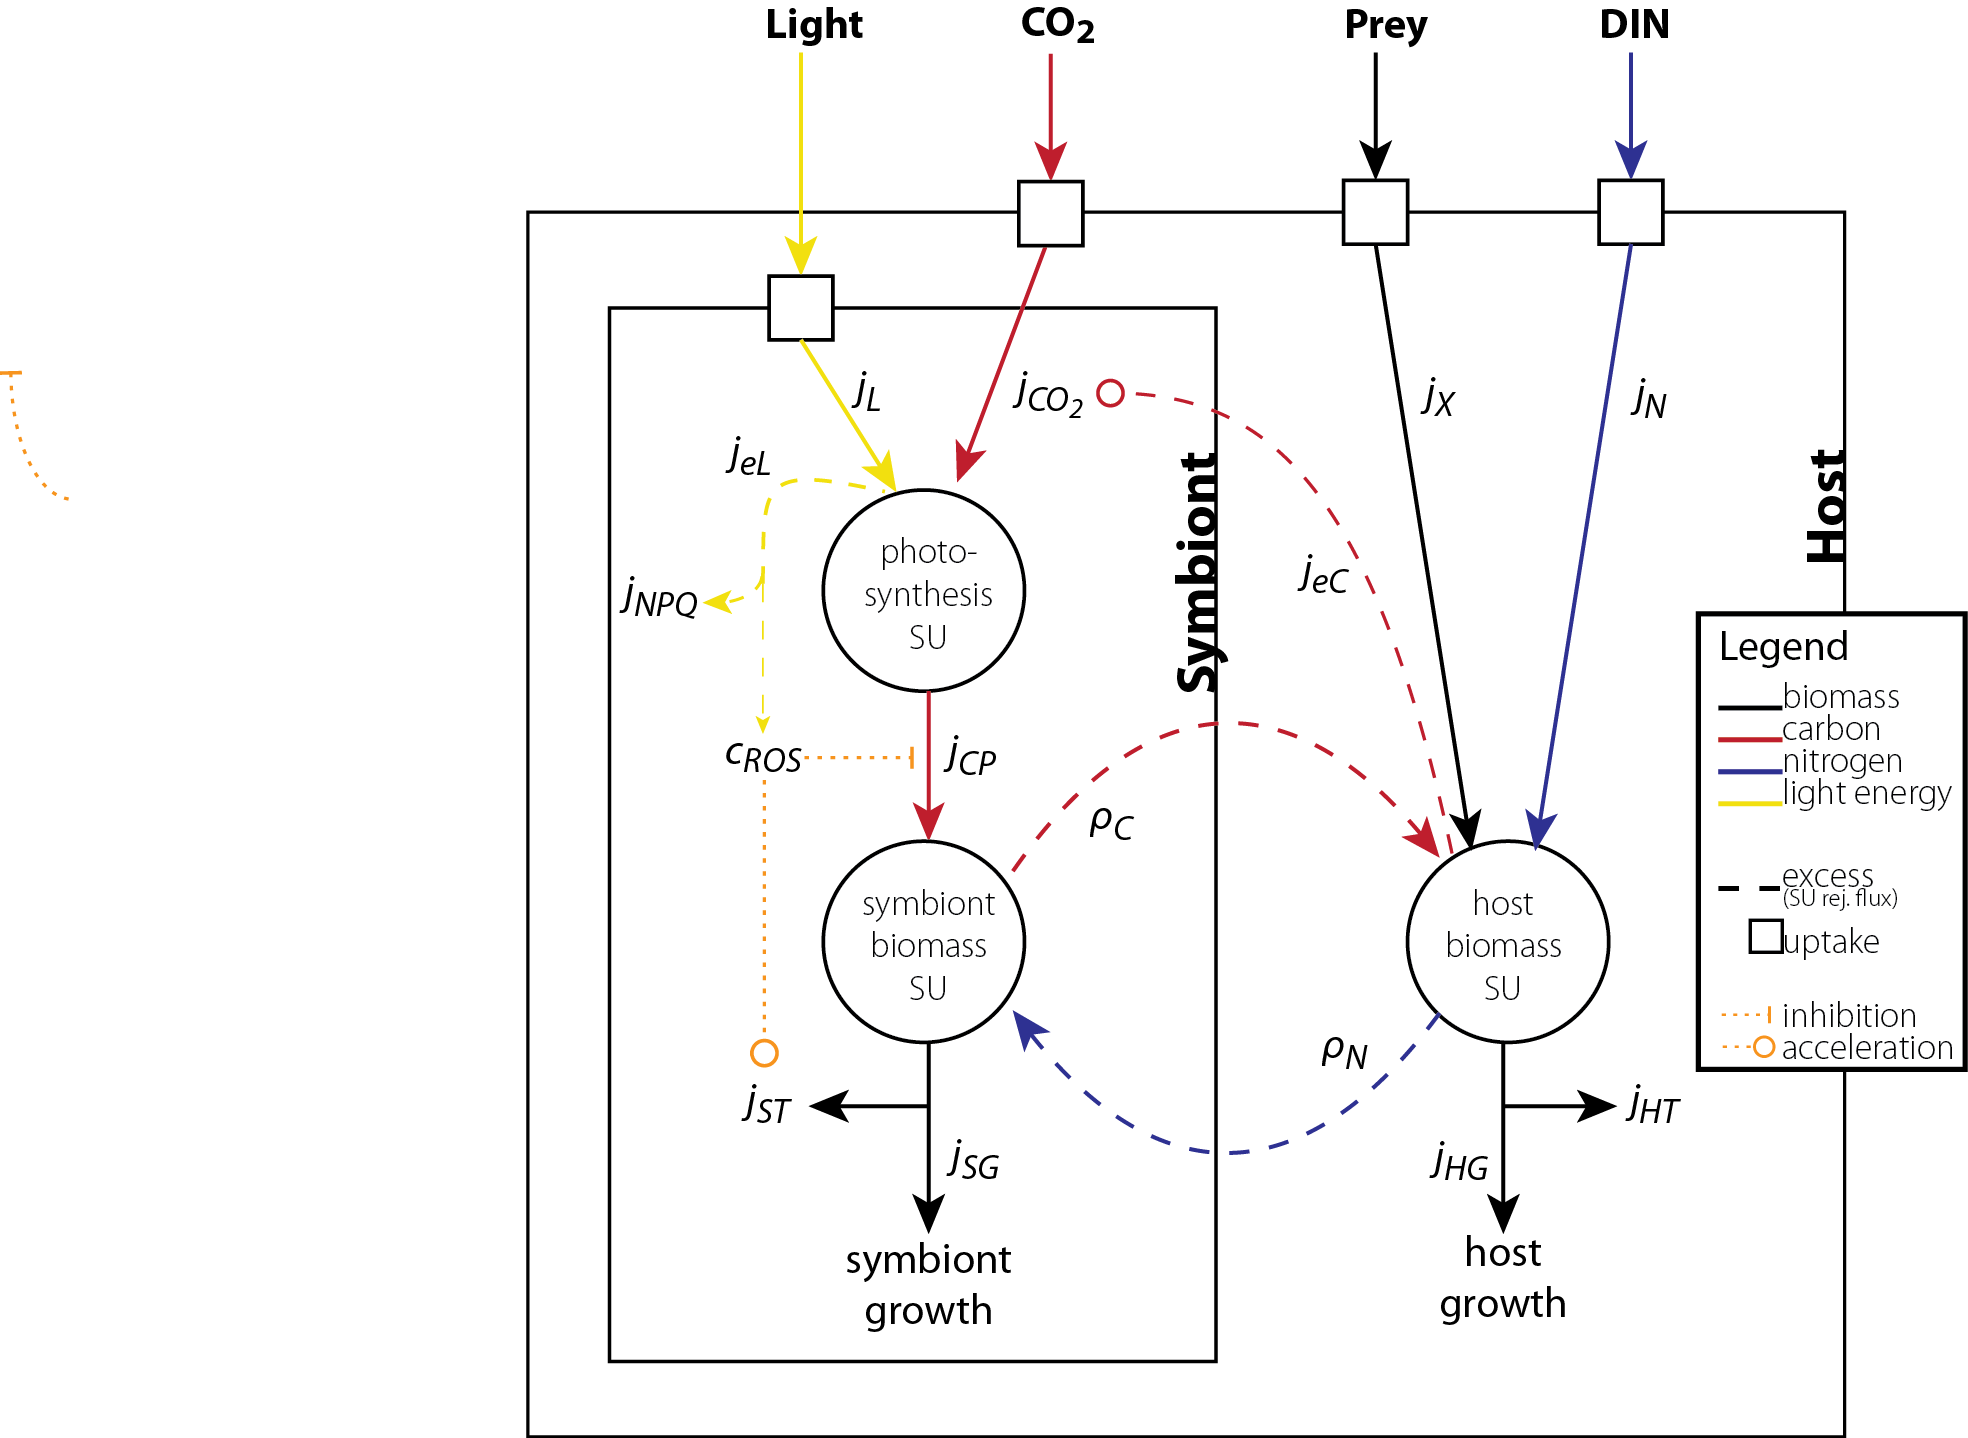
\includegraphics{../img/Fig1.png}
\caption{Graphical representation of coral-algal symbiosis model. Light,
CO\textsubscript{2}, prey, and DIN are acquired from the external
environment proportional to the biomass of the partner indicated by the
black box for uptake. Mass fluxes (see Table 1 for definitions) are
represented by \(j\)'s with subscripts indicating the type of mass, and
in some cases the process (e.g., \(j_{CP}\) is the flux of carbon
produced by photosynthesis), and \(\rho\)'s indicate fluxes that are
shared by one partner with the other. Parallel complementary
synthesizing units (SUs) are represented by large circles, and rejection
fluxes from these SUs are indicated by dashed lines. \(c_{ROS}\) is a
proportional rate that impacts other model fluxes by inhibition or
acceleration; likewise, \(j_{eC}\) accelerates the rate of \(j_{CO_2}\).
Recycled mass fluxes from biomass turnover are not shown for clarity
(but see Table 1 for definitions).}
\end{figure}

\subsection{State equations}\label{state-equations}

The balance equations for symbiont and host biomass are expressed as:

\begin{equation} {dS \over Sdt} = j_{SG} - j_{ST} \end{equation}

\begin{equation} {dH \over Hdt} = j_{HG} - j_{HT}^0 \end{equation}

These are expressed per unit of symbiont and host biomass, respectively.
The specific biomass growth and turnover rates that define these balance
equations are produced by combinations of the individual model fluxes
(see Table 1 for definitions and units), which are each expressed as
mass-specific rates (e.g., per C-mole of symbiont or host biomass). When
necessary, conversions between symbiont-mass-specific and
host-mass-specific rates are accomplished by multiplying or dividing by
the symbiont:host biomass ratio.

\subsection{Coral animal fluxes}\label{coral-animal-fluxes}

The coral animal acquires both carbon and nitrogen from feeding on prey
from the environment. Prey acquisition is specified by Michaelis-Menten
kinetics (i.e., a Holling type II function) with a maximum feeding rate
\(j_{Xm}\) and half-saturation constant \(K_X\):

\begin{equation} j_X = {{j_{Xm} \cdot X} \over {X + K_X}} \end{equation}

Additionally, the coral animal acquires nitrogen dissolved in the
surrounding seawater, which is assumed to represent ammonium, the
primary form utilized by corals (Yellowlees, Rees, and Leggat 2008).
This gives the host (rather than the symbiont) priority in nitrogen
utilization; this capacity is supported by experimental evidence (Wang
and Douglas 1998) and is consistent with the physical arrangment of the
partners, where the host is in direct contact with the external
environment. The uptake of nitrogen from the environment is thus
specified by Michaelis-Menten kinetics using a maximum uptake rate
\(j_{Nm}\) and half-saturation constant \(K_N\):

\begin{equation} j_N = {{j_{Nm} \cdot N} \over {N + K_N}} \end{equation}

Coral biomass formation is then specified by a parallel complementary SU
that combines carbon and nitrogen, according to:

\begin{equation} j_{HG} = \bigg({1 \over j_{HGm}} + {1 \over {\rho_C{S \over H} + j_X}} + {1 \over {(j_N + n_{NX}j_X + r_{NH}) / n_{NH}}} - {1 \over {{\rho_C{S \over H} + j_X} + (j_N + n_{NX}j_X + r_{NH}) / n_{NH}}}\bigg)^{-1} \end{equation}

where \(\rho_C\) is the surplus fixed carbon shared by the symbiont (see
below), and \(r_{NH}\) is the recycled portion of the nitrogen liberated
by host biomass turnover:

\begin{equation} r_{NH}=\sigma_{NH}n_{NH}j_{HT}^0 \end{equation}

The amount of nitrogen input to the coral biomass SU in excess of what
is actually consumed in biomass formation (i.e., surplus nitrogen, or
the rejection flux\footnote{Rejection fluxes must always be positive,
  and hence are specified with the notation \((x)_+\), which means
  \(max(x, 0)\).} of the SU) is then made available to the symbiont:

\begin{equation} \rho_N = (j_N + n_{NX}j_X + r_{NH} - n_{NH}j_{HG})_+ \end{equation}

The carbon rejected from this SU reflects the amount of excess fixed
carbon available to the host that is not used in biomass formation:

\begin{equation} j_{eC} = (jX + \rho_C{S \over H} - j_{HG})_+ \end{equation}

This flux, \(j_{eC}\), is assumed to be available as a respiratory
substrate to support various energetically-demanding processes; of
particular importance is the host's active supply of CO\textsubscript{2}
for symbiont photosynthesis (Wooldridge 2013; Hopkinson, Tansik, and
Fitt 2015) (see below).

Due to the inherent inefficiency of the parallel complementary SU
formulation, there is always some nitrogen shared with the symbiont even
when coral biomass formation is strongly nitrogen-limited. Likewise,
there is always a non-zero rejection flux of excess carbon from the
coral biomass SU.

\subsection{\texorpdfstring{\emph{Symbiodinium}
fluxes}{Symbiodinium fluxes}}\label{symbiodinium-fluxes}

The symbiont produces fixed carbon through photosynthesis, a process
represented here by a single SU with two substrates: light (photons) and
inorganic carbon (CO\textsubscript{2}). The amount of light absorbed by
the symbiont depends on the scalar irradiance at the site of light
absorption, which is modified substantially relative to external
downwelling irradiance owing to multiple scattering by the coral
skeleton and self-shading by surrounding symbionts (Enríquez, Méndez,
and Iglesias-Prieto 2005; Marcelino et al. 2013). We used data from
Marcelino et al. (2013) to empirically derive an amplification factor,
\(A\), indicating the ratio of internal scalar irradiance to external
downwelling irradiance as a function of symbiont density (S:H biomass),
which is specified as:

\begin{equation} A = 1.26 + 1.39 \cdot \exp(-6.48 \cdot {S \over H}) \end{equation}

This amplification factor is then multiplied by the external downwelling
irradiance \(L\) and the effective light-absorbing surface area of
symbiont biomass \(\bar{a}^*\) to specify the total light absorption:

\begin{equation} j_L =  A \cdot L \cdot \bar{a}^* \end{equation}

We then specify the input of CO\textsubscript{2} to photosynthesis as
\(j_{CO_2}\), a flux mediated by the host that encompasses potentially
diverse carbon-concentrating mechanisms (CCMs), including active
transport of bicarbonate, carbonic anhydrase-catalyzed conversion of
bicarbonate to CO\textsubscript{2} to promote diffusion toward the
symbiont (Tansik, Fitt, and Hopkinson 2015), and acidification of the
symbiosome to increase localized CO\textsubscript{2} concentrations
around the symbiont (Barott et al. 2014). Since these mechanisms require
energetic input by the host, the magnitude of CO\textsubscript{2}
delivery is proportional to the host's excess carbon, \(j_{eC}\),
assuming that some of this carbon is respired to energize these CCMs.
This formulation means that the symbiont indirectly ensures its own
CO\textsubscript{2} supply by providing fixed carbon to the host
(Wooldridge 2013), which establishes a positive feedback in the model
that leads to the existence of multiple stable states, which we discuss
below in the context of coral bleaching. The parameter \(k_{CO_2}\)
scales the efficacy of host CCMs, which enables the comparison of
different rates of CO\textsubscript{2} delivery that may characterize
different coral species (Wooldridge 2014a). The input of
CO\textsubscript{2} to the photosynthesis SU is therefore specified as:

\begin{equation} j_{CO_2} = k_{CO_2}j_{eC} \end{equation}

Additional metabolic CO\textsubscript{2} recycled from both the host and
symbiont biomass turnover is also made available to the photosynthesis
SU, according to:

\begin{equation} r_{CH}=\sigma_{CH}j_{HT}^0 \end{equation}\begin{equation} r_{CS}=\sigma_{CS}j_{ST}^0 \end{equation}

Fixed carbon is then produced by the photosynthesis SU according to:

\begin{equation} j_{CP} = \bigg({1 \over j_{CPm}} + {1 \over {y_{CL} j_L }} + {1 \over {(j_{CO_2} + r_{CH}){H \over S} + r_{CS}}} - {1 \over {y_{CL} j_L + (j_{CO_2} + r_{CH}){H \over S} + r_{CS}}}\bigg)^{-1} \cdot c_{ROS}^{-1} \end{equation}

where \(j_{CPm}\) is the maximum specific rate of photosynthesis, and
\(c_{ROS}\) is the relative rate of reactive oxygen species production
(see below). Dividing the photosynthetic rate by \(c_{ROS}\) causes a
decline in response to photooxidative stress at high light levels, and
the emergent outcome of this SU formulation demonstrates a classic
photoinhibition response (see Fig. S1).

Light energy absorbed in excess of what is used to fix carbon is
specified by the SU ``rejection flux'', according to:

\begin{equation} j_{eL} = (j_L - j_{CP} / y_{CL})_+ \end{equation}

This excess light energy must be quenched by alternative pathways in
order to prevent photooxidative damage (Powles 1984).
\emph{Symbiodinium} utilize a variety of pathways for non-photochemical
quenching (NPQ; Roth 2014), which we collect in a relative NPQ capacity
specified as a parameter of the symbiont (\(k_{NPQ}\)). The total NPQ
flux is specified as a single-substrate SU formula:

\begin{equation} j_{NPQ} = \bigg({1 \over k_{NPQ}} + {1 \over j_{eL}}\bigg)^{-1} \end{equation}

If light energy further exceeds the capacity of both photochemistry and
NPQ, then reactive oxygen species (ROS) are produced. We represent this
as a relative quantity \(c_{ROS}\), taking a value of 1 when all light
energy is quenched by photochemistry and NPQ, and increasing as the
amount of excess excitation energy increases:

\begin{equation} c_{ROS} = 1 + {{(j_{eL} - j_{NPQ})_+} \over k_{ROS}} \end{equation}

where \(k_{ROS}\) is a parameter of the symbiont that determines the
rate of ROS production (specifically, the amount of excess excitation
energy that doubles ROS production relative to baseline levels).
Importantly, \(c_{ROS}\) is specified here not as a function of absolute
external light, but rather the amount of excess light, \(j_{eL}\), after
accounting for quenching by carbon fixation and NPQ. A direct
consequence of this formulation is that CO\textsubscript{2}-limitation
of photosynthesis can lead to ROS production, an important mechanism
(Wooldridge 2009) that was not captured by previous representations of
photooxidative stress (Eynaud, Nisbet, and Muller 2011).

Carbon fixed by photosynthesis (\(j_{CP}\)) is then combined with
nitrogen shared by the host (\(\rho_N\)) and nitrogen recycled from
symbiont biomass turnover

\begin{equation} r_{NS}=\sigma_{NS}n_{NS}j_{ST}^0 \end{equation}

to build new symbiont biomass, following the SU equation:

\begin{equation} j_{SG} = \bigg({1 \over j_{SGm}} + {1 \over j_{CP}} + {1 \over {(\rho_N{H \over S} + r_{NS}) / n_{NH}}} - {1 \over {j_{CP} + (\rho_N{H \over S} + r_{NS}) / n_{NH}}}\bigg)^{-1} \end{equation}

The rejection flux of carbon from this SU represents the amount of fixed
carbon produced by photosynthesis in excess of what can be used to
produce symbiont biomass; this surplus, \(\rho_C\), is translocated to
the coral host:

\begin{equation} \rho_C = (j_{CP} - j_{SG})_+ \end{equation}

The rejection flux of nitrogen from the symbiont biomass SU is lost to
the environment.

Symbiont biomass turnover includes a component of constant turnover
specified by the parameter \(j_{ST}^0\), representing fixed maintenance
costs, plus a component that scales with the magnitude of ROS
production.

\begin{equation} j_{ST} = j_{ST}^0(1 + b(c_{ROS}-1)) \end{equation}

This second component of symbiont biomass loss represents both
photodamage and/or symbiont expulsion (i.e., bleaching), both of which
occur in response to high levels of ROS production. The parameter \(b\)
is included to scale biomass loss due to bleaching in response to ROS.
(Note that recycling of symbiont biomass turnover (\(rNS\) and \(rCS\))
only occurs based on the maintenance component of turnover (i.e.,
\(j_{ST}^0\)), and not the bleaching-related component, as this loss
represents biomass that is damaged or expelled from the host.)

\subsection{Numerical analysis}\label{numerical-analysis}

A time-stepping Euler method was used to solve the state equations since
the production and rejection fluxes of the SUs are imiplicitly defined
due to feedbacks present in the model. Specifically, the rejection
fluxes of carbon and nitrogen from the symbiont and host biomass SUs act
as reciprocal input fluxes to the other SU. In addition, the
photosynthesis SU receives CO\textsubscript{2} proportional to the
carbon rejection flux from the host biomass SU, and the rejection flux
of excitation energy from the photosynthesis SU acts to reduce its own
production (i.e., photoinhibition). A vector of time steps is used for
each simulation, along which dynamic environmental forcing functions
(irradiance, DIN, and prey abundance) can be designed. These vectors,
along with initial values of symbiont and host biomass, then serve as
input to the time-stepping function, which solves for the current system
state using values of the previous system state where necessary. A time
step of 0.1 days was used for all simulations, which were performed
using R code that is available in the data repository accompanying this
article: \url{github.com/jrcunning/Rcoral}.

To aid in visualizing model results, we calculated values to indicate
the degree to which product formation at an SU was limited by
availability of either of its two substrates:

\begin{equation} \log \bigg({{\min(j_{S1}, j_{Pm})} \over {\min(j_{S2}, j_{Pm})}}\bigg) \end{equation}

where \(j_{S1}\) and \(j_{S2}\) are the specific input fluxes of the two
substrates and \(j_{Pm}\) is the maximum specific product formation
rate, in units of Cmol Cmol\textsuperscript{-1} d\textsuperscript{-1}.

\section{Results}\label{results}

\subsection{Qualitative dynamics}\label{qualitative-dynamics}

In a constant environment, the system ultimately reaches a steady state
of exponential growth or decline. Under some conditions, alternate
steady states can be reached depending on initial values of symbiont and
host biomass. The mechanism that produces these alternate steady states
is the positive feedback between carbon-limitation of the host and
CO\textsubscript{2}-limitation of photosynthesis. If the host becomes
carbon-limited, the efficacy of its CCMs are reduced and photosynthesis
becomes progressively more CO\textsubscript{2}-limited. In turn, less
photosynthate is translocated to the host, causing further
carbon-limitation and an ultimate decline in biomass; this steady state
represents a dysfunctional symbiosis. However, if the host is not
carbon-limited, it effectively delivers CO\textsubscript{2} to
photosynthesis and ensures its continued receipt of fixed carbon from
the symbiont; this system is nitrogen-limited and represents a
functional symbiosis with positive exponential growth. Either of these
stable states may be reached under (some sets of) constant environmental
conditions, depending on the initial values of symbiont and host
biomass: if symbiont biomass is initially very low (i.e., a ``bleached''
coral), the system cannot escape the carbon-limited state and cannot
grow. However, if symbiont biomass is initially high (i.e., a healthy
coral), then the system maintains positive growth in a nitrogen-limited
state. For practical purposes, we consider only positive growth steady
states in the ``steady state behavior'' section below. In the subsequent
``dynamic behavior'' section, we explore more thoroughly the conditions
that cause the system to switch between alternate stable states, and
interpret these dynamics in the context of coral bleaching.

\subsection{Steady state behavior}\label{steady-state-behavior}

To analyze qualitative behavior, we ran the model to steady state across
gradients of external irradiance and nutrients (Fig. 2), which revealed
patterns consistent with observed phenomena in corals. Predicted growth
rates are low at low light and DIN (\textasciitilde{}0.01
d\textsuperscript{-1}), and begin increasing as both of these factors
increase (Fig. 2A). Low light is limiting to photosynthesis (Fig. 2D),
which leads to carbon-limitation of host growth (Fig. 2B) and an
associated increase in the symbiont to host biomass ratio (Fig. 2C). In
agreement with this trend are many observations of negative correlation
between irradiance and symbiont density (Stimson 1997; Brown et al.
1999; Fitt et al. 2000; Titlyanov et al. 2001). As higher light
alleviates light-limitation of photosynthesis, growth becomes less
carbon-limited. Similarly, elevating DIN up to \textasciitilde{}2 µM
alleviates nitrogen-limitation (Fig. 2B). Increased growth at higher DIN
is predicted by the DEB model of Muller et al. (2009), and has also been
observed experimentally (Muller-Parker et al. 1994; Tanaka et al. 2007;
Tanaka et al. 2013). However, DIN elevation beyond a certain point
(e.g., \textasciitilde{}3-4 µM in these simulations) has little effect
on growth as carbon becomes limiting (Fig. 2B). Very high nutrient
levels may even reduce growth (Shantz, Lemoine, and Burkepile 2015),
although these impacts are not likely to occur within the range of
concentrations considered here (\textless{}4 µM) (Ferrier-Pagès et al.
2000).

In addition to increasing growth, DIN also increases the symbiont to
host biomass ratio, a phenomenon also observed in reef corals (Marubini
and Davies 1996). S:H ratios also increase under low light (Stimson
1997; Fitt et al. 2000; Anthony and Hoegh-Guldberg 2003). At low DIN and
intermediate light, more typical of coral reef environments, symbiont to
host biomass ratios are around \textasciitilde{}0.1-0.3, which is
consistent with values reported in the literature (Muscatine, R
McCloskey, and E Marian 1981; Edmunds et al. 2011).

\begin{figure}[htbp]
\centering
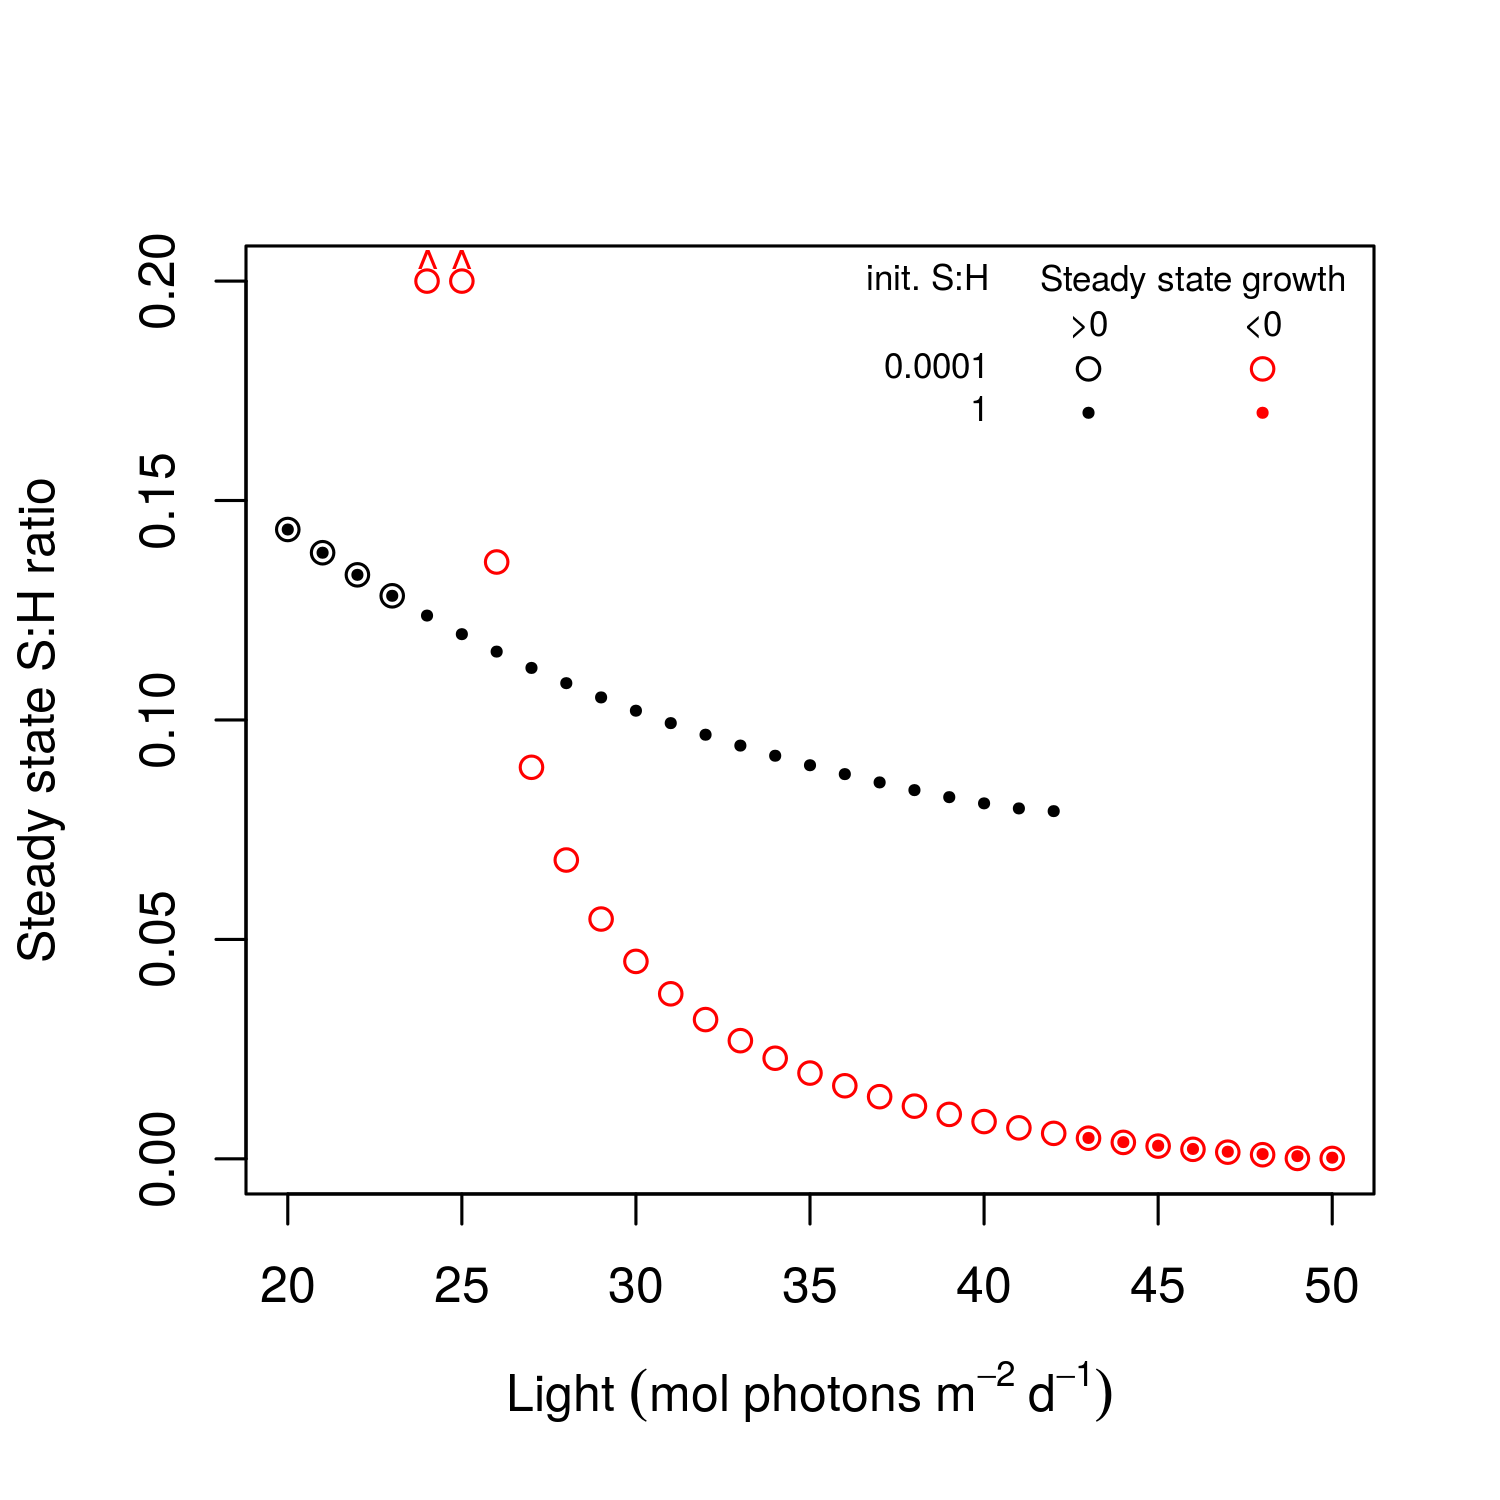
\includegraphics{../img/Fig2.png}
\caption{Steady state values of \textbf{A)} specific growth (Cmol
Cmol\textsuperscript{-1} d\textsuperscript{-1}), \textbf{B)} the
symbiont to host biomass ratio (CmolS CmolH\textsuperscript{-1}),
\textbf{C)} relative C- or N-limitation of host biomass formation, and
\textbf{D)} relative CO\textsubscript{2}- or light-limitation of
symbiont photosynthesis, across gradients of external irradiance and
dissolved inorganic nitrogen. Note that typical conditions for reefs are
\textasciitilde{}1e-7 M DIN and 10-20 mol photons m\textsuperscript{-2}
d\textsuperscript{-1}. Simulations for each combination of light and
nutrients (41 points along each axis) were run for 100 days with a time
step of 1 day. Negative steady state growth rates, and corresponding S:H
ratios, were set to zero.}
\end{figure}

The maximum predicted growth rates of \textasciitilde{}0.1
d\textsuperscript{-1}, occurring between \textasciitilde{}10-20 mol
photons m\textsuperscript{-2} s\textsuperscript{-1} light and
\textasciitilde{}4 µM DIN (Fig. 2A), are comparable to the rate of 0.07
d\textsuperscript{-1} measured by Tanaka et al. (2007) under similar
N-enriched conditions. Growth under conditions more typical of reef
environments (\textless{}0.5 µM DIN) are within the range of
\textasciitilde{}0.01-0.03 d\textsuperscript{-1}; these values are
slightly higher than most specific growth rates reported in the
literature, which are typically based on skeletal mass, and fall near or
below 0.01 d\textsuperscript{-1} (Osinga et al. 2011; Osinga et al.
2012) (though values as high as 0.025 d\textsuperscript{-1} have been
reported (Schutter et al. 2010)). These generally low skeletal growth
rates relative to predicted biomass growth may be explained by
differential substrate-limitation (i.e., CO\textsubscript{2} may limit
calcification, which is not present in the model); indeed, tissue and
skeletal growth may not always be well correlated (Anthony 2002).
Furthermore, bioerosion may reduce net skeletal growth, especially in
the field (Bak 1976). Nevertheless, when rates of increase in coral
tissue biomass have been directly measured over short periods, values
are consistent with model predictions (e.g., 0.07 d\textsuperscript{-1}
in Tanaka et al. (2007)), and similar rates (0.04 d\textsuperscript{-1})
have been measured in \emph{Aiptasia diaphana}, a non-calcifying
symbiotic anemone (Armoza-Zvuloni et al. 2014).

As irradiance continues to increase above \textasciitilde{}20 mol
photons m\textsuperscript{-2} d\textsuperscript{-1}, growth rates
decline until positive growth ceases above \textasciitilde{}35 µmol
photons m\textsuperscript{-2} d\textsuperscript{-1}. The mechanism
underlying this decline is the increase in light energy beyond the
capacity of photosynthesis and non-photochemical quenching: excess
excitation energy generates reactive oxygen species (ROS) (Weis 2008;
Roth 2014), which, in this model, have the phenomenological consequences
of reducing the photosynthetic rate (representing photoinhibition) and
increasing symbiont biomass loss (representing photodamage and/or
symbiont expulsion) (see Eynaud, Nisbet, and Muller 2011). Together,
these impacts reduce the symbiont to host biomass ratio (Fig. 2C), as
occurs during coral bleaching. This reduction in symbionts consequently
reduces the flux of fixed carbon to the host, resulting in increasing
carbon-limitation (Fig. 2B) and eventual cessation of growth (Fig. 2A).
Importantly, these consequences arise in the present model only when
light energy exceeds the capacity of photochemistry and NPQ, which in
turn depends on CO\textsubscript{2} availability. While previous models
framed photophysiological stress as a fixed response to absolute
irradiance levels (Eynaud, Nisbet, and Muller 2011), the current
implementation considers the dynamic balance of multiple energy sinks in
the causation of stress, which is more consistent with current
understanding of symbiosis dysfunction (Wooldridge 2013), and
establishes an important role of the host in providing
CO\textsubscript{2} for symbiont photosynthesis (Tansik, Fitt, and
Hopkinson 2015; Hopkinson, Tansik, and Fitt 2015).

While bleaching in response to high light alone has been observed
experimentally (Schutter et al. 2011; Downs et al. 2013), mass coral
bleaching events occur in response to high temperature (Hoegh-Guldberg
1999); thus, it is important to justify our consideration of light as
the primary stressor in the model. In reality, light and temperature
interact synergistically (Coles and Jokiel 1978; Jones et al. 1998), and
in fact, any stressor that disrupts the quenching of light energy may
lead to bleaching (Wooldridge 2010; Baker and Cunning 2015). This is
because the proximate cause of coral bleaching is excess excitation
energy, but the upstream events that lead to this situation may be
diverse: indeed, elevated temperature inhibits Rubisco functioning
(Jones et al. 1998) and repair of the D1 protein in photosystem II
(Warner, Fitt, and Schmidt 1999), which reduces the capacity of
photochemical quenching and leads to an excess of light energy. In this
way, elevated temperature serves to reduce the threshold above which
light causes stress to the system (Hoegh-Guldberg 1999); importantly,
light is still the proximate stressor. Therefore, we omitted temperature
from the model, which serves to maintain a desired level of simplicity,
while still allowing photophysiological stress and bleaching to be
simulated with biological realism in response to light. Thus, the
specific light levels that cause stress here should be interpreted in
this context, and the effects of high light are analagous to the effects
of high temperature.

The incorporation of light stress in the model sets an upper limit to
the amount of light at which a stable symbiotic interaction can be
maintained, but even below this threshold of breakdown, negative effects
of high light reduce steady state growth and symbiont:host biomass (Fig.
2A,C). This gradual decline is consistent with experimental results
showing that high light levels decrease growth (Schutter et al. 2011),
and field studies documenting optimum growth rates at intermediate
depths (Baker and Weber 1975; Huston 1985). Consequently, the model
predicts greater variation in state variables across light gradients
than was predicted by the model of Muller et al. (2009), which did not
include photoinhibition and photodamage. It is important to recognize
that these are steady state values predicted under a constant
environment at the given light and nutrient levels; a dynamic system may
temporarily cross this threshold and experience a period of symbiont
loss (bleaching) and reduced growth, after which a return to benign
conditions may restore symbiont biomass and positive growth. To explore
this further and illustrate the behavior of the model in more detail, we
evaluate a number of dynamic simulations below.

\subsection{Sensitivity analysis -- should come after the steady states
bc describes changes in steady
states}\label{sensitivity-analysis-should-come-after-the-steady-states-bc-describes-changes-in-steady-states}

Each default parameter value used in the model (Table 2) is based on
carefully selected relevant literature. A supplementary document
detailing the derivations of each of these default parameter values is
provided. Nevertheless, it is important to evaluate the sensitivity of
the model to changes in these parameter values. We measured fractional
change in steady state values in response to fractional change in
parameter values, relative to their default values (Table 2).

\begin{figure}[htbp]
\centering
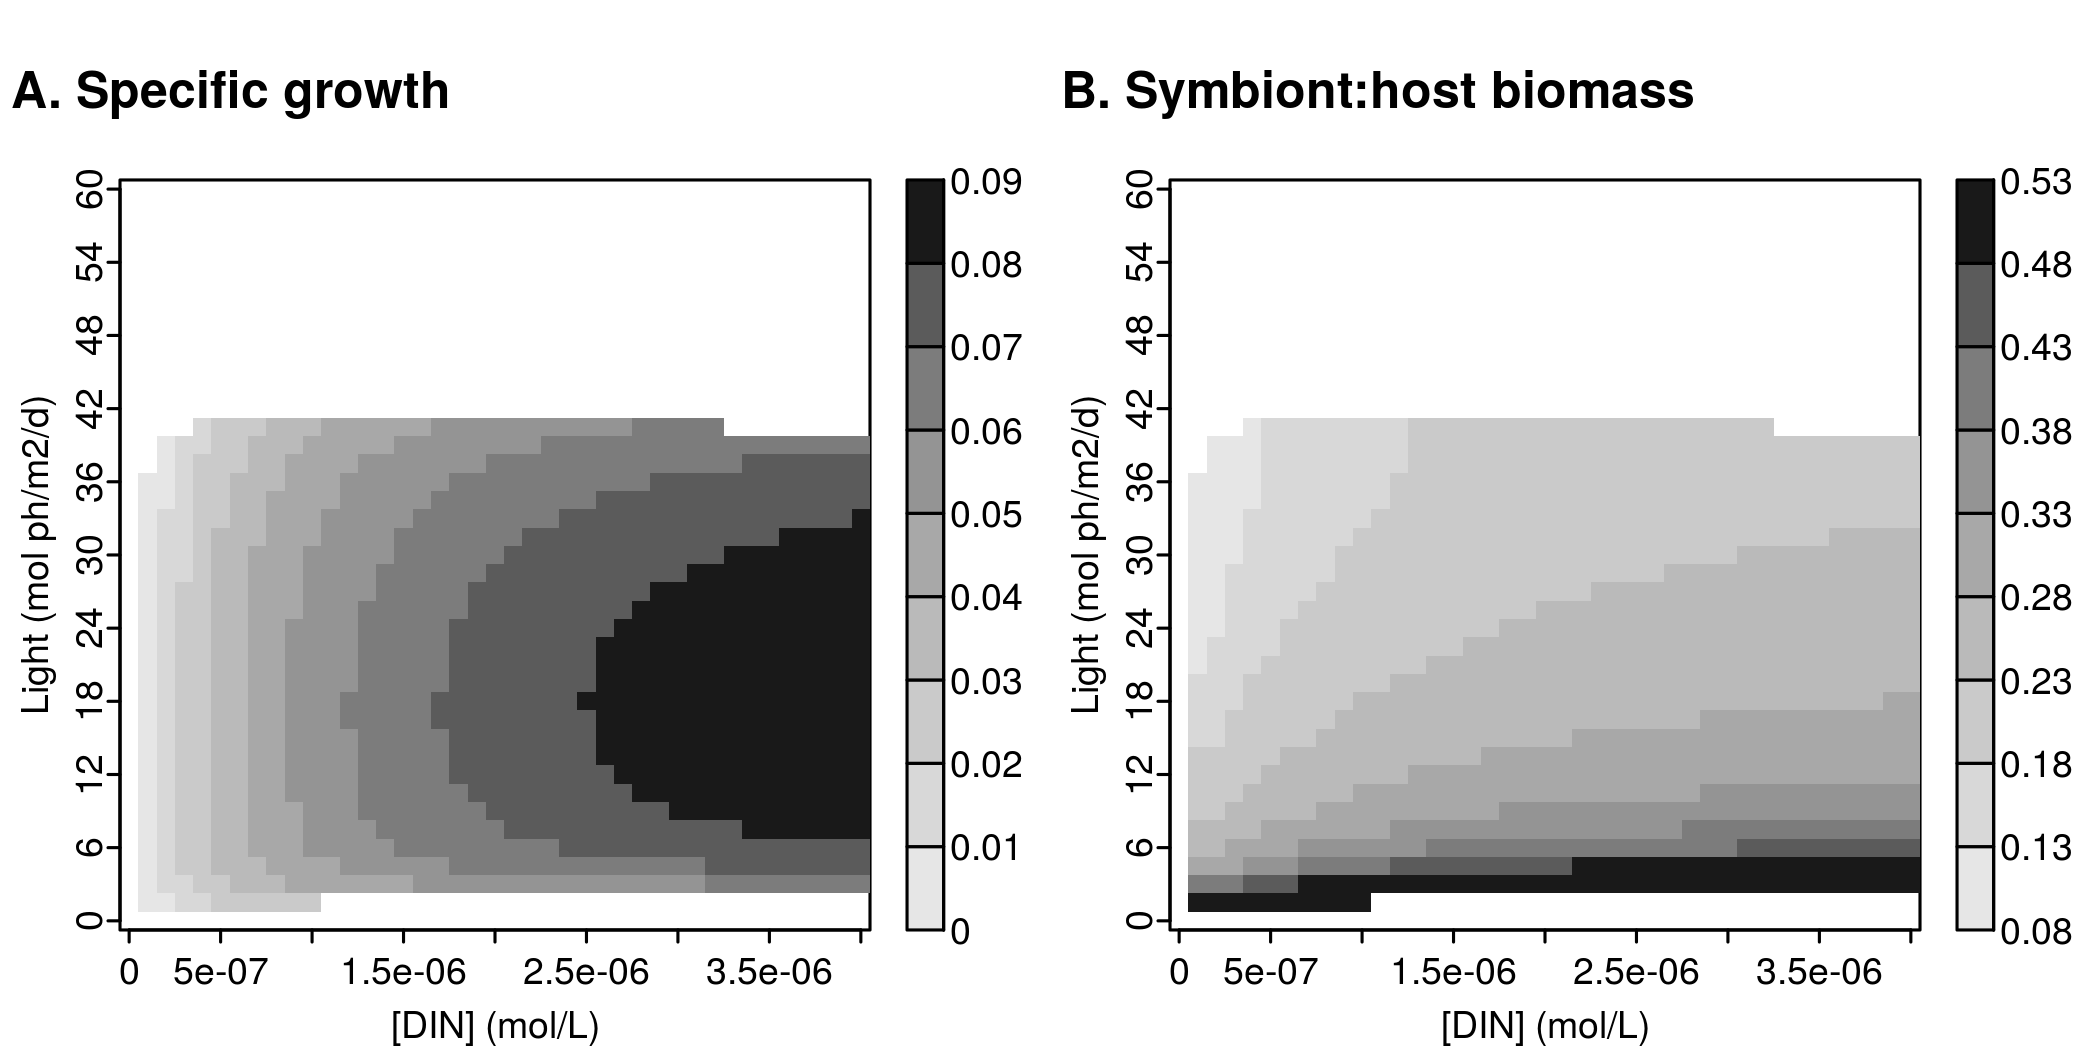
\includegraphics{../img/Fig3.png}
\caption{Sensitivity analysis. Plots show the fractional change in
steady state values of growth (solid lines) and S:H biomass (dashed
lines) in response to fractional changes in default parameter values
(see Table 2 for default values). Parameters are grouped by which
processes they are involved in. This sensitivity analysis was conducted
at conditions typical for coral reef environments: low DIN (1e-7 M) and
intermediate light (15 mol m\textsuperscript{-2} d\textsuperscript{-2}).
Sensitivity analyses conducted other environmental conditions are
presented in the Supplementary Information.}
\end{figure}

\subsection{Dynamic behavior}\label{dynamic-behavior}

Therefore, we are highly interested in the conditions under which the
system switches from one state to another, representing the conditions
under which corals ``bleach'' due to progressive, reinforcing
carbon-limitation. Interestingly, this state can be reached in multiple
ways, by the acceleration of photoinhibition and photodamage, or by high
external DIN, which causes the symbiont to share less carbon,
subsequently causing its own CO2-limitation, and progressive
C-limitation of the system. \#\# varying light: consequences of excess
light and light-limitation \#\# varying DIN: role of N-limitation and
consequences of elevated N \#\# elevated nutrients cause system to
become C-limited (photo: CO2 limited; host: fixed-C limited) \#\#
C-limitation increases susceptibility to bleaching \#\# consequences of
a less efficient but more tolerant symbiont \#\# Rate of symbiont
repopulation (Berner et al. 1993) \#\# Bicarbonate addition promotes
coral growth (Marubini and Thake 1999) \#\# Seasonal change in sym.
density is larger when nutrients are elevated (Stimson 1997). Such a
phenomenon was predicted by Fitt et al. 2000. \#\# Death rule: negative
growth for a certain amount of time should be defensible.

\section*{References}\label{references}
\addcontentsline{toc}{section}{References}

\hypertarget{refs}{}
\hypertarget{ref-Anthony:2002tc}{}
Anthony, K. 2002. ``Comparative analysis of energy allocation to tissue
and skeletal growth in corals.'' \emph{Limnology and Oceanography} 47
(5): 1417--29.
\url{https://www.scopus.com/inward/record.uri?partnerID=HzOxMe3b\&scp=0036733455\&origin=inward}.

\hypertarget{ref-Anthony:2003p3632}{}
Anthony, Kenneth R N, and Ove Hoegh-Guldberg. 2003. ``Variation in coral
photosynthesis, respiration and growth characteristics in contrasting
light microhabitats: an analogue to plants in forest gaps and
understoreys?'' \emph{Functional Ecology} 17 (April): 246--59.

\hypertarget{ref-ArmozaZvuloni:2014ju}{}
Armoza-Zvuloni, Rachel, Esti Kramarsky-Winter, Yossi Loya, Ami
Schlesinger, and Hanna Rosenfeld. 2014. ``Trioecy, a unique breeding
strategy in the sea anemone Aiptasia diaphana and its association with
sex steroids.'' \emph{Biology of Reproduction} 90 (6). Society for the
Study of Reproduction: 122--22.
doi:\href{https://doi.org/10.1095/biolreprod.113.114116}{10.1095/biolreprod.113.114116}.

\hypertarget{ref-Bak:1976bv}{}
Bak, R. 1976. ``The growth of coral colonies and the importance of
crustose coralline algae and burrowing sponges in relation with
carbonate accumulation.'' \emph{Netherlands Journal of Sea Research} 10
(3): 285--337.
doi:\href{https://doi.org/10.1016/0077-7579(76)90009-0}{10.1016/0077-7579(76)90009-0}.

\hypertarget{ref-Baker:2015kp}{}
Baker, Andrew C, and Ross Cunning. 2015. ``Coral 'Bleaching' as a
Generalized Stress Response to Environmental Disturbance.'' In
\emph{Diseases of Coral}, 396--409. Hoboken, NJ: John Wiley \& Sons,
Inc.
doi:\href{https://doi.org/10.1002/9781118828502.ch30}{10.1002/9781118828502.ch30}.

\hypertarget{ref-Baker:1975ip}{}
Baker, P, and Jon N Weber. 1975. ``Coral growth rate: Variation with
depth.'' \emph{Earth and Planetary Science Letters} 27 (1): 57--61.
doi:\href{https://doi.org/10.1016/0012-821X(75)90160-0}{10.1016/0012-821X(75)90160-0}.

\hypertarget{ref-Barott:2014gx}{}
Barott, Katie L, Alexander A Venn, Sidney O Perez, Sylvie Tambutte, and
Martin Tresguerres. 2014. ``Coral host cells acidify symbiotic algal
microenvironment to promote photosynthesis.'' \emph{Proceedings Of The
National Academy Of Sciences Of The United States Of America}, December.
National Acad Sciences, 201413483.
doi:\href{https://doi.org/10.1073/pnas.1413483112}{10.1073/pnas.1413483112}.

\hypertarget{ref-Brown:1999p3534}{}
Brown, Barbara E, R P Dunne, I Ambarsari, Martin Le Tissier, and U
Satapoomin. 1999. ``Seasonal fluctuations in environmental factors and
variations in symbiotic algae and chlorophyll pigments in four
Indo-Pacific coral species.'' \emph{Marine Ecology Progress Series} 191:
53--69.

\hypertarget{ref-Coles:1978p1124}{}
Coles, SL, and Paul L Jokiel. 1978. ``Synergistic effects of
temperature, salinity and light on the hermatypic coral Montipora
verrucosa.'' \emph{Marine Biology} 49: 187--95.
\url{http://www.springerlink.com/index/LU582837924G7674.pdf}.

\hypertarget{ref-Costanza:2014ex}{}
Costanza, R, R de Groot, and P Sutton. 2014. ``Changes in the global
value of ecosystem services.'' \emph{Global Environmental Change} 26:
152--58.
doi:\href{https://doi.org/10.1016/j.gloenvcha.2014.04.002}{10.1016/j.gloenvcha.2014.04.002}.

\hypertarget{ref-Downs:2013kc}{}
Downs, C A, Kathleen E McDougall, Cheryl M Woodley, John E Fauth, Robert
H Richmond, Ariel Kushmaro, Stuart W Gibb, Yossi Loya, Gary K Ostrander,
and Esti Kramarsky-Winter. 2013. ``Heat-Stress and Light-Stress Induce
Different Cellular Pathologies in the Symbiotic Dinoflagellate during
Coral Bleaching.'' \emph{PLoS ONE} 8 (12): e77173.
doi:\href{https://doi.org/10.1371/journal.pone.0077173}{10.1371/journal.pone.0077173}.

\hypertarget{ref-Edmunds:2011bv}{}
Edmunds, Peter J, Hollie M Putnam, Roger M Nisbet, and Erik B Muller.
2011. ``Benchmarks in organism performance and their use in comparative
analyses.'' \emph{Oecologia} 167 (2): 379--90.
doi:\href{https://doi.org/10.1007/s00442-011-2004-2}{10.1007/s00442-011-2004-2}.

\hypertarget{ref-Enriquez:2005p142}{}
Enríquez, Susana, Eugenio R Méndez, and Roberto Iglesias-Prieto. 2005.
``Multiple scattering on coral skeletons enhances light absorption by
symbiotic algae.'' \emph{Limnology and Oceanography} 50 (4): 1025--32.

\hypertarget{ref-Eynaud:2011tv}{}
Eynaud, Yoan, Roger M Nisbet, and Erik B Muller. 2011. ``Impact of
excess and harmful radiation on energy budgets in scleractinian
corals.'' \emph{Ecological Modelling} 222 (7). Elsevier: 1315--22.
\url{http://www.sciencedirect.com/science/article/pii/S0304380011000263}.

\hypertarget{ref-FerrierPages:2000p1950}{}
Ferrier-Pagès, Christine, Jean-Pierre Gattuso, S Dallot, and Jean
Jaubert. 2000. ``Effect of nutrient enrichment on growth and
photosynthesis of the zooxanthellate coral Stylophora \ldots{}.''
\emph{Coral Reefs}.
\url{http://www.springerlink.com/index/3DRC3K1Q57TPC0UT.pdf}.

\hypertarget{ref-Fitt:2000p3792}{}
Fitt, William K, F K McFarland, Mark E Warner, and Geoff C Chilcoat.
2000. ``Seasonal patterns of tissue biomass and densities of symbiotic
dinoflagellates in reef corals and relation to coral bleaching.''
\emph{Limnology and Oceanography} 45 (3): 677--85.

\hypertarget{ref-Glynn:2001p7571}{}
Glynn, Peter W, Juan L Maté, Andrew C Baker, and MO Calderón. 2001.
``Coral bleaching and mortality in Panama and Ecuador during the
1997-1998 El Niño-Southern Oscillation event: Spatial/temporal patterns
and comparisons with the 1982-1983 event.'' \emph{Bulletin of Marine
Science} 69 (1): 79--109.

\hypertarget{ref-HoeghGuldberg:1999p4222}{}
Hoegh-Guldberg, Ove. 1999. ``Climate change, coral bleaching and the
future of the world's coral reefs.'' \emph{Marine and Freshwater
Research} 50 (November): 839--66.

\hypertarget{ref-Hopkinson:2015ev}{}
Hopkinson, Brian M, Anna L Tansik, and William K Fitt. 2015. ``Internal
carbonic anhydrase activity in the tissue of scleractinian corals is
sufficient to support proposed roles in photosynthesis and
calcification.'' \emph{The Journal of Experimental Biology}, April. The
Company of Biologists Ltd, jeb.118182.
doi:\href{https://doi.org/10.1242/jeb.118182}{10.1242/jeb.118182}.

\hypertarget{ref-Huston:1985ec}{}
Huston, M. 1985. ``Variation in coral growth rates with depth at
Discovery Bay, Jamaica.'' \emph{Coral Reefs} 4 (1): 19--25.
doi:\href{https://doi.org/10.1007/BF00302200}{10.1007/BF00302200}.

\hypertarget{ref-Jager:2013bj}{}
Jager, Tjalling, Benjamin T Martin, and Elke I Zimmer. 2013. ``DEBkiss
or the quest for the simplest generic model of animal life history.''
\emph{Journal of Theoretical Biology} 328: 9--18.
doi:\href{https://doi.org/10.1016/j.jtbi.2013.03.011}{10.1016/j.jtbi.2013.03.011}.

\hypertarget{ref-Jokiel:1977p7353}{}
Jokiel, Paul L, and SL Coles. 1977. ``Effects of temperature on the
mortality and growth of Hawaiian reef corals.'' \emph{Marine Biology} 43
(3): 201--8.

\hypertarget{ref-Jones:1998p3572}{}
Jones, Ross J, Ove Hoegh-Guldberg, Anthony W D Larkum, and Ulrich
Schreiber. 1998. ``Temperature-induced bleaching of corals begins with
impairment of the CO2 fixation mechanism in zooxanthellae.''
\emph{Plant, Cell and Environment} 21 (12): 1219--30.

\hypertarget{ref-Kooijman:2010vd}{}
Kooijman, SALM. 2010. \emph{Dynamic Energy Budget Theory for Metabolic
Organization}. 3rd ed. Cambridge University Press.

\hypertarget{ref-Marcelino:2013hz}{}
Marcelino, Luisa A, Mark W Westneat, Valentina Stoyneva, Jillian Henss,
Jeremy D Rogers, Andrew Radosevich, Vladimir Turzhitsky, et al. 2013.
``Modulation of Light-Enhancement to Symbiotic Algae by Light-Scattering
in Corals and Evolutionary Trends in Bleaching.'' \emph{PLoS ONE} 8 (4):
e61492.
doi:\href{https://doi.org/10.1371/journal.pone.0061492.s008}{10.1371/journal.pone.0061492.s008}.

\hypertarget{ref-Marubini:1996p8460}{}
Marubini, F, and PS Davies. 1996. ``Nitrate increases zooxanthellae
population density and reduces skeletogenesis in corals.'' \emph{Marine
Biology} 127 (2): 319--28.
\url{http://www.scopus.com/inward/record.url?partnerID=yv4JPVwI\&eid=2-s2.0-0030301761\&md5=0971551a6865f30046294b9e17fb4081}.

\hypertarget{ref-Muller:2009io}{}
Muller, Erik B, Sebastiaan A L M Kooijman, Peter J Edmunds, Francis J
Doyle, and Roger M Nisbet. 2009. ``Dynamic energy budgets in syntrophic
symbiotic relationships between heterotrophic hosts and photoautotrophic
symbionts.'' \emph{Journal of Theoretical Biology} 259 (1): 44--57.
doi:\href{https://doi.org/10.1016/j.jtbi.2009.03.004}{10.1016/j.jtbi.2009.03.004}.

\hypertarget{ref-MullerParker:1994uo}{}
Muller-Parker, Gisèle, Lawrence R McCloskey, Ove Hoegh-Guldberg, and PJ
McAuley. 1994. ``Effect of ammonium enrichment on animal and algal
biomass of the coral Pocillopora damicornis.'' \emph{Pacific Science} 48
(3). \url{http://scholarspace.manoa.hawaii.edu/handle/10125/2236}.

\hypertarget{ref-Muscatine:1977p4220}{}
Muscatine, Leonard, and James W Porter. 1977. ``Reef corals: mutualistic
symbioses adapted to nutrient-poor environments.'' \emph{Bioscience} 27
(7): 454--60.

\hypertarget{ref-Muscatine:1981jy}{}
Muscatine, Leonard, L R McCloskey, and R E Marian. 1981. ``Estimating
the daily contribution of carbon from zooxanthellae to coral animal
respiration.'' \emph{Limnology and Oceanography} 26 (4): 601--11.
doi:\href{https://doi.org/10.4319/lo.1981.26.4.0601}{10.4319/lo.1981.26.4.0601}.

\hypertarget{ref-Osinga:2011kq}{}
Osinga, Ronald, Miriam Schutter, Ben Griffioen, René H Wijffels, Johan A
J Verreth, Shai Shafir, Stéphane Henard, Maura Taruffi, Claudia Gili,
and Silvia Lavorano. 2011. ``The Biology and Economics of Coral
Growth.'' \emph{Marine Biotechnology} 13 (4): 658--71.
doi:\href{https://doi.org/10.1007/s10126-011-9382-7}{10.1007/s10126-011-9382-7}.

\hypertarget{ref-Osinga:2012is}{}
Osinga, Ronald, Miriam Schutter, Tim Wijgerde, Buki Rinkevich, Shai
Shafir, Muki Shpigel, Gian Marco Luna, et al. 2012. ``The CORALZOO
project: a synopsis of four years of public aquarium science.''
\emph{Journal of the Marine Biological Association of the UK} 92 (04).
Cambridge University Press: 753--68.
doi:\href{https://doi.org/10.1017/S0025315411001779}{10.1017/S0025315411001779}.

\hypertarget{ref-Powles:1984tm}{}
Powles, Stephen B. 1984. ``Photoinhibition of photosynthesis induced by
visible light.'' \emph{Annual Review of Plant Physiology} 35: 15--44.

\hypertarget{ref-RALanguageandEn:2014wf}{}
R Core Team. 2014. ``R: A Language and Environment for Statistical
Computing.'' Vienna, Austria: R Foundation for Statistical Computing.
\url{http://www.R-project.org/}.

\hypertarget{ref-Roth:2014wf}{}
Roth, M S. 2014. ``The engine of the reef: Photobiology of the
coral-algal symbiosis.'' \emph{Frontiers in Microbiology}.
\url{http://journal.frontiersin.org/Journal/10.3389/fmicb.2014.00422/pdf}.

\hypertarget{ref-Schutter:2010p7758}{}
Schutter, M, J Crocker, A Paijmans, M Janse, R Osinga, A J Verreth, and
R H Wijffels. 2010. ``The effect of different flow regimes on the growth
and metabolic rates of the scleractinian coral Galaxea fascicularis.''
\emph{Coral Reefs}, April.
doi:\href{https://doi.org/10.1007/s00338-010-0617-2}{10.1007/s00338-010-0617-2}.

\hypertarget{ref-Schutter:2011ie}{}
Schutter, Miriam, Rosa M van der Ven, Max Janse, Johan A J Verreth, René
H Wijffels, and Ronald Osinga. 2011. ``Light intensity, photoperiod
duration, daily light flux and coral growth of Galaxea fascicularis in
an aquarium setting: a matter of photons?'' \emph{Journal of the Marine
Biological Association of the UK} 92 (04). Cambridge University Press:
703--12.
doi:\href{https://doi.org/10.1017/S0025315411000920}{10.1017/S0025315411000920}.

\hypertarget{ref-Shantz:2015dz}{}
Shantz, Andrew A, Nathan P Lemoine, and Deron E Burkepile. 2015.
``Nutrient loading alters the performance of key nutrient exchange
mutualisms.'' \emph{Ecology Letters} 19 (1): 20--28.
doi:\href{https://doi.org/10.1111/ele.12538}{10.1111/ele.12538}.

\hypertarget{ref-Stimson:1997p3837}{}
Stimson, J. 1997. ``The annual cycle of density of zooxanthellae in the
tissues of field and laboratory-held Pocillopora damicornis
(Linnaeus).'' \emph{Journal of Experimental Marine Biology and Ecology}
214 (1-2): 35--48.

\hypertarget{ref-Tanaka:2013dj}{}
Tanaka, Yasuaki, Akira Iguchi, Mayuri Inoue, Chiharu Mori, K Sakai,
Atsushi Suzuki, Hodaka Kawahata, and Takashi Nakamura. 2013. ``Marine
Pollution Bulletin.'' \emph{Marine Pollution Bulletin} 68 (1-2): 93--98.
doi:\href{https://doi.org/10.1016/j.marpolbul.2012.12.017}{10.1016/j.marpolbul.2012.12.017}.

\hypertarget{ref-Tanaka:2007uv}{}
Tanaka, Yasuaki, Toshihiro Miyajima, Isao Koike, Takeshi Hayashibara,
and Hiroshi Ogawa. 2007. ``Imbalanced coral growth between organic
tissue and carbonate skeleton caused by nutrient enrichment.''
\emph{Limnology and Oceanography}.
\url{http://www.aslo.org/lo/toc/vol_52/issue_3/1139.pdf}.

\hypertarget{ref-Tansik:2015cm}{}
Tansik, Anna L, William K Fitt, and Brian M Hopkinson. 2015. ``External
carbonic anhydrase in three Caribbean corals: quantification of activity
and role in CO2 uptake.'' \emph{Coral Reefs} 34 (3). Springer Berlin
Heidelberg: 703--13.
doi:\href{https://doi.org/10.1007/s00338-015-1289-8}{10.1007/s00338-015-1289-8}.

\hypertarget{ref-Titlyanov:2001p3631}{}
Titlyanov, E A, T V Titlyanova, K Yamazato, and Robert van Woesik. 2001.
``Photo-acclimation dynamics of the coral Stylophora pistillata to low
and extremely low light.'' \emph{Journal of Experimental Marine Biology
and Ecology} 263 (2): 211--25.

\hypertarget{ref-Wang:1998p128}{}
Wang, J, and Angela E Douglas. 1998. ``Nitrogen recycling or nitrogen
conservation in an alga-invertebrate symbiosis?'' \emph{The Journal of
Experimental Biology} 201: 2445--53.

\hypertarget{ref-Warner:1999p4239}{}
Warner, Mark E, William K Fitt, and Gregory W Schmidt. 1999. ``Damage to
photosystem II in symbiotic dinoflagellates: A determinant of coral
bleaching.'' \emph{Proceedings Of The National Academy Of Sciences Of
The United States Of America} 96 (14): 8007--12.

\hypertarget{ref-Weis:2008p944}{}
Weis, Virginia M. 2008. ``Cellular mechanisms of Cnidarian bleaching:
stress causes the collapse of symbiosis.'' \emph{The Journal of
Experimental Biology} 211 (Pt 19): 3059--66.
doi:\href{https://doi.org/10.1242/jeb.009597}{10.1242/jeb.009597}.

\hypertarget{ref-Wooldridge:2009p7807}{}
Wooldridge, Scott A. 2009. ``A new conceptual model for the warm-water
breakdown of the coral-algae endosymbiosis.'' \emph{Marine and
Freshwater Research} 60 (June): 483--96.

\hypertarget{ref-Wooldridge:2010p7809}{}
---------. 2010. ``Is the coral-algae symbiosis really 'mutually
beneficial' for the partners?'' \emph{BioEssays}, May.

\hypertarget{ref-Wooldridge:2013tj}{}
---------. 2013. ``Breakdown of the coral-algae symbiosis: towards
formalising a linkage between warm-water bleaching thresholds and the
growth rate of the intracellular zooxanthellae.'' \emph{Biogeosciences}
10: 1647--58.
\url{http://www.biogeosciences.net/10/1647/2013/bg-10-1647-2013.html}.

\hypertarget{ref-Wooldridge:2014di}{}
---------. 2014a. ``Differential thermal bleaching susceptibilities
amongst coral taxa: re-posing the role of the host.'' \emph{Coral Reefs}
33 (1). Springer Berlin Heidelberg: 15--27.
doi:\href{https://doi.org/10.1007/s00338-013-1111-4}{10.1007/s00338-013-1111-4}.

\hypertarget{ref-Wooldridge:2014hc}{}
---------. 2014b. ``Formalising a mechanistic linkage between
heterotrophic feeding and thermal bleaching resistance.'' \emph{Coral
Reefs}. Springer Berlin Heidelberg, 1--6.
doi:\href{https://doi.org/10.1007/s00338-014-1193-7}{10.1007/s00338-014-1193-7}.

\hypertarget{ref-Yellowlees:2008p331}{}
Yellowlees, David, T A V Rees, and William Leggat. 2008. ``Metabolic
interactions between algal symbionts and invertebrate hosts.''
\emph{Plant, Cell and Environment} 31: 679--94.

\end{document}


